% Este archivo es parte de la memoria del proyecto fin de carrera
% de Manuel López Urbina. Protegida bajo la licencia GFDL.
% Para más información, la licencia completa viene incluida en el
% fichero fdl-1.3.tex

% Copyright (C) 2012 Manuel López Urbina

\chapter{Software de control}
\label{chap:software-de-control}

En presente capítulo contiene información relativa a las herramientas software utilizadas y desarrolladas para la realización de la comunicación con el vehículo ordenando acciones como movimientos, modificación de velocidad, entre otros. Todo ello desde el ordenador por parte del usuario.\\

Cabe recordar que la aplicación consta de dos modos de funcionamiento; un modo automático donde los movimientos son realizados a partir de los elementos visionados por la cámara, y un segundo modo donde el vehículo es manejable por el usuario. En este tema de desarrollan ambos aspectos.\\

Para el control del vehículo se ha utilizado un software denominado \emph{Surveyor Robot Software} \footnote{Para la descarga de código fuente visite el siguiente enlace \url{{http://agents.sci.brooklyn.cuny.edu/robotics.edu/bcsoftware.php}}.}, el cual ha sido desarrollado por John Cummins junto con los agentes de laboratorio de la Universidad de Brooklyn con la asistencia de M.P. Azhar, y la supervisión del profesor Sklar empleando el lenguaje de programación C++. El código está liberado bajo Copyleft.\\

El código \emph{Surveyor robot software} ha sido ligeramente modificado para adaptarlo a las necesidades del proyecto, la principal modificación añadida ha sido la de añadir un método para permitir la conexión y desconexión con el vehículo. Permitiendo al usuario desconectar y reconectar a su antojo.

\section{Control por parte del usuario}

Lo interesante era proporcionar una serie de mecanismos que permitiera mantener un control del vehículo de una manera cómoda y eficaz para el usuario. Los elementos proporcionados para realizar el control del vehículo son el uso del teclado del ordenador y un gamepad.

\subsection{Control desde teclado}

Los movimientos clásicos del vehículo, avance, retroceso y giros, han sido ordenados mediante el uso de las teclas de dirección. Para las capturas de los eventos desde el teclado se han utilizado las herramientas proporcionadas por la biblioteca Qt.\\

De este modo, el vehículo, al presionar la tecla de avance, comenzaba a andar, pero no se detenía hasta nueva orden haciendo incómodo su manejo. Como solución al problema se optó por capturar el evento de ``soltado'' de tecla para, en ese instante, mandar una orden de detención de tal manera que el vehículo avance sólo y exclusivamente mientras se encuentra la tecla pulsada.\\

Por otro lado, el robot SRV-1, al tratarse de un vehículo tipo tanque, presenta la particularidad de poder controlar las velocidades de movimiento de los motores de un mismo lateral por igual permitiendo la realización de giros. Como consecuencia de lo anterior, si se aplica una velocidad levemente inferior en un lateral que en el otro el vehículo realizará un giro muy abierto. De modo contrario, si detenemos por completo los motores de un lado, el giro producido será de pequeña amplitud. Esta circunstancia permite que desde las flechas de teclado no podamos controlar tal efecto, puesto que los giros serán siempre iguales, que para el caso de las teclas de dirección será únicamente moviendo los motores de un lateral.\\

\begin{figure}[H]
  \begin{center}
    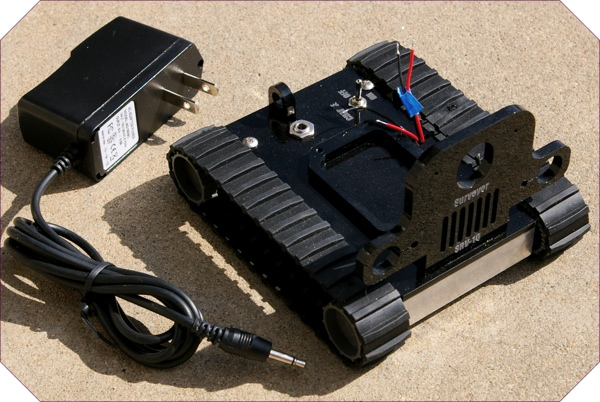
\includegraphics[scale=0.5]{quad-base.jpg}
  \end{center}
  \caption{Visualización del chasis del robot y su sistema de desplazamiento tipo tanque.}
  \label{fig:quad-base}
\end{figure}

 Para permitir realizar ambos tipos de giros se pensó en capturar combinaciones de teclas, de tal modo que si se presiona la tecla ``derecha'', el vehículo realice un giro cerrado y si se presiona la tecla ``arriba'' más ``derecha'', el giro será de mayor amplitud. Los diferentes movimientos existentes en el vehículo quedan descritos en la sección \ref{sec:uso-teclado} del manual.\\

Para su realización, Qt no dispone de los elementos necesarios para capturar combinaciones de teclas, solamente es posible con las teclas ``Shift'', ``Ctrl'',`` Alt'' y ``Meta''.\\

Como solución al problema de la captura de eventos múltiples se implementó un buffer donde se almacenaba un identificador de las dos últimas teclas pulsadas, eliminándose un identificador del buffer en el momento en que la tecla sea soltada. De ese modo tras la captura de un evento, se analizaba el estado del buffer y se determinaba la orden de movimiento a realizar. Obteniendo los movimientos descritos en la sección \ref{sec:uso-teclado} del manual.\\

En la siguiente imagen podemos ver una representación gráfica del comportamiento del buffer de control del vehículo:\\

\begin{figure}[H]
  \begin{center}
    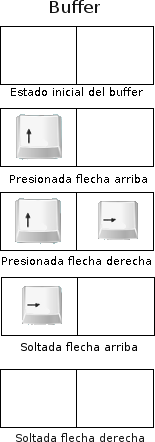
\includegraphics[scale=0.8]{buffer-teclado2.png}
  \end{center}
  \caption{Representación del funcionamiento del buffer creado para la captura de eventos múltiples.}
  \label{fig:buffer-teclado}
\end{figure}


\subsection{Control mediante gamepad}

Para hacer más cómodo, aún si cabe, el manejo del vehículo, se decidió incorporar un mando o gamepad, para ello ha sido necesaria la utilización de la biblioteca SDL con el fin de detectar el dispositivo y capturar los eventos correspondientes no presentando dificultades destacables. Para ver los controles fijados vea sección \ref{sec:convencion-gamepad} de la guía de usuario.

\section{Control automático}

Para dotar al vehículo de un sistema de conducción autónoma se han diseñado una serie de respuestas automáticas ordenadas cuando una determinada señal es detectada. En esta sección se describen cada una de ellas.\\

Entre el conjunto de señales de tráfico reconocibles por el sistema disponemos de las indicadoras de velocidad máxima. Estas señales detectables varían desde los 20 hasta los 100 km/h. Cuando una determinada velocidad es detectada, ésta debe ser asignada al vehículo con la finalidad de realizar los movimientos de una manera proporcional a la velocidad indicadora de la señal reconocida. \\

La biblioteca \emph{Surveyor Robot Software} permite ajustar las velocidades de movimiento del vehículo en una escala desde el 0 hasta el 100. Por tanto, si la señal de tráfico detectada se corresponde con la de 50km/h, se asigna al vehículo un valor de velocidad de 50.\\

En el momento de la detección de la señal de Stop, se ordena su detención manteniéndose intacto el valor de velocidad que se encuentra en ese momento fijado.\\

Para las señales correspondientes a las indicadoras de dirección obligatoria (flechas), se efectúa un giro de manera automática. En la sección \ref{sec:operaciones-automatizadas} del manual se muestra al detalle los diferentes movimientos realizados para cada señal de tráfico detectada.\\

Por otro lado, cuando una señal es detectada, la orden automatizada es enviada al vehículo una sola vez de tal modo que si en el entorno apareciese más adelante la misma señal reconocida anteriormente, ésta no se volverá a realizar. En definitiva, no se reconoce la misma señal de tráfico dos veces seguidas. \\

\begin{figure}[H]
  \begin{center}
    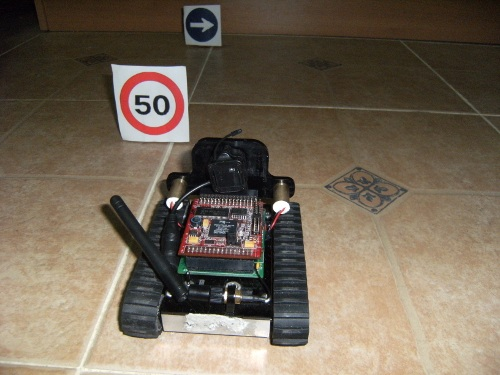
\includegraphics[scale=0.8]{circuito.jpg}
  \end{center}
  \caption{Fotografía de un circuito realizable por el vehículo .}
  \label{fig:circuito}
\end{figure}


A continuación se muestra el código realizado para la realización de los movimientos autónomos. En ella se analiza un vector para comprobar si contiene los identificadores de las clases de aquellos objetos que se correspondan con una señal. Por ejemplo, si el vector contiene los identificadores ``2'' y ``0'' determinamos que el elemento detectado es una señal de 20 km/h.\\

\underline{Código para el control automatizado del vehículo}
\begin{Verbatim}[commandchars=\\\{\}]
\PY{k+kt}{int}  \PY{n}{MainWindow}\PY{o}{:}\PY{o}{:}\PY{n}{accion\PYZus{}SVR}\PY{p}{(}\PY{n}{std}\PY{o}{:}\PY{o}{:}\PY{n}{vector}\PY{o}{<}\PY{k+kt}{char}\PY{o}{>} \PY{o}{&}\PY{n}{v}\PY{p}{)}\PY{p}{\PYZob{}}


    \PY{c+c1}{// 100 km/h}
    \PY{k}{if} \PY{p}{(}\PY{p}{(}\PY{n}{std}\PY{o}{:}\PY{o}{:}\PY{n}{find}\PY{p}{(}\PY{n}{v}\PY{p}{.}\PY{n}{begin}\PY{p}{(}\PY{p}{)}\PY{p}{,} \PY{n}{v}\PY{p}{.}\PY{n}{end}\PY{p}{(}\PY{p}{)}\PY{p}{,}\PY{l+s+sc}{'1'}\PY{p}{)}\PY{o}{!}\PY{o}{=} \PY{n}{v}\PY{p}{.}\PY{n}{end}\PY{p}{(}\PY{p}{)}\PY{p}{)} \PY{o}{&}\PY{o}{&}
        \PY{p}{(}\PY{n}{std}\PY{o}{:}\PY{o}{:}\PY{n}{find}\PY{p}{(}\PY{n}{v}\PY{p}{.}\PY{n}{begin}\PY{p}{(}\PY{p}{)}\PY{p}{,} \PY{n}{v}\PY{p}{.}\PY{n}{end}\PY{p}{(}\PY{p}{)}\PY{p}{,}\PY{l+s+sc}{'0'}\PY{p}{)} \PY{o}{!}\PY{o}{=} \PY{n}{v}\PY{p}{.}\PY{n}{end}\PY{p}{(}\PY{p}{)}\PY{p}{)}\PY{p}{)}\PY{p}{\PYZob{}}

        \PY{c+c1}{// Se elimina un '0'.}
        \PY{n}{std}\PY{o}{:}\PY{o}{:}\PY{n}{vector}\PY{o}{<}\PY{k+kt}{char}\PY{o}{>}\PY{o}{:}\PY{o}{:}\PY{n}{iterator} \PY{n}{pos} \PY{o}{=} \PY{n}{std}\PY{o}{:}\PY{o}{:}\PY{n}{find}\PY{p}{(}\PY{n}{v}\PY{p}{.}\PY{n}{begin}\PY{p}{(}\PY{p}{)}\PY{p}{,} \PY{n}{v}\PY{p}{.}\PY{n}{end}\PY{p}{(}\PY{p}{)}\PY{p}{,}\PY{l+s+sc}{'0'}\PY{p}{)}\PY{p}{;}
        \PY{n}{v}\PY{p}{.}\PY{n}{erase}\PY{p}{(}\PY{n}{pos}\PY{p}{)}\PY{p}{;}

        \PY{c+c1}{// Si existe otro cero...}
        \PY{k}{if}\PY{p}{(}\PY{n}{std}\PY{o}{:}\PY{o}{:}\PY{n}{find}\PY{p}{(}\PY{n}{v}\PY{p}{.}\PY{n}{begin}\PY{p}{(}\PY{p}{)}\PY{p}{,} \PY{n}{v}\PY{p}{.}\PY{n}{end}\PY{p}{(}\PY{p}{)}\PY{p}{,}\PY{l+s+sc}{'0'}\PY{p}{)}\PY{o}{!}\PY{o}{=} \PY{n}{v}\PY{p}{.}\PY{n}{end}\PY{p}{(}\PY{p}{)}\PY{p}{)}\PY{p}{\PYZob{}}

            \PY{c+c1}{// 100 km/h}
            \PY{k}{if}\PY{p}{(}\PY{n}{conectado} \PY{o}{&}\PY{o}{&} \PY{n}{ui}\PY{o}{-}\PY{o}{>}\PY{n}{checkBox\PYZus{}2}\PY{o}{-}\PY{o}{>}\PY{n}{isChecked}\PY{p}{(}\PY{p}{)} \PY{o}{&}\PY{o}{&} \PY{n}{ultima\PYZus{}senial} \PY{o}{!}\PY{o}{=} \PY{l+m+mi}{10}\PY{p}{)}\PY{p}{\PYZob{}}
                \PY{n}{ultima\PYZus{}senial} \PY{o}{=} \PY{l+m+mi}{10}\PY{p}{;}
                \PY{n}{robot}\PY{p}{.}\PY{n}{move}\PY{p}{(}\PY{n}{STOP}\PY{p}{)}\PY{p}{;}
                \PY{n}{this}\PY{o}{-}\PY{o}{>}\PY{n}{velocidad} \PY{o}{=} \PY{l+m+mi}{100}\PY{p}{;}
                \PY{n}{robot}\PY{p}{.}\PY{n}{drive}\PY{p}{(}\PY{n}{this}\PY{o}{-}\PY{o}{>}\PY{n}{velocidad}\PY{p}{,}\PY{n}{this}\PY{o}{-}\PY{o}{>}\PY{n}{velocidad}\PY{p}{)}\PY{p}{;}
            \PY{p}{\PYZcb{}}
            \PY{c+c1}{//Mostrar señal detectada}
            \PY{n}{mostrar\PYZus{}senial\PYZus{}detectada}\PY{p}{(}\PY{l+s}{"}\PY{l+s}{10.jpg}\PY{l+s}{"}\PY{p}{)}\PY{p}{;}

            \PY{k}{return} \PY{l+m+mi}{0}\PY{p}{;}
        \PY{p}{\PYZcb{}}
    \PY{p}{\PYZcb{}}


    \PY{c+c1}{// 20 km/h}
    \PY{k}{if} \PY{p}{(}\PY{p}{(}\PY{n}{std}\PY{o}{:}\PY{o}{:}\PY{n}{find}\PY{p}{(}\PY{n}{v}\PY{p}{.}\PY{n}{begin}\PY{p}{(}\PY{p}{)}\PY{p}{,} \PY{n}{v}\PY{p}{.}\PY{n}{end}\PY{p}{(}\PY{p}{)}\PY{p}{,}\PY{l+s+sc}{'2'}\PY{p}{)} \PY{o}{!}\PY{o}{=} \PY{n}{v}\PY{p}{.}\PY{n}{end}\PY{p}{(}\PY{p}{)}\PY{p}{)} \PY{o}{&}\PY{o}{&} 
        \PY{p}{(}\PY{n}{std}\PY{o}{:}\PY{o}{:}\PY{n}{find}\PY{p}{(}\PY{n}{v}\PY{p}{.}\PY{n}{begin}\PY{p}{(}\PY{p}{)}\PY{p}{,} \PY{n}{v}\PY{p}{.}\PY{n}{end}\PY{p}{(}\PY{p}{)}\PY{p}{,}\PY{l+s+sc}{'0'}\PY{p}{)} \PY{o}{!}\PY{o}{=} \PY{n}{v}\PY{p}{.}\PY{n}{end}\PY{p}{(}\PY{p}{)}\PY{p}{)}\PY{p}{)}\PY{p}{\PYZob{}}

        \PY{k}{if}\PY{p}{(}\PY{n}{conectado} \PY{o}{&}\PY{o}{&} \PY{n}{ui}\PY{o}{-}\PY{o}{>}\PY{n}{checkBox\PYZus{}2}\PY{o}{-}\PY{o}{>}\PY{n}{isChecked}\PY{p}{(}\PY{p}{)} \PY{o}{&}\PY{o}{&} \PY{n}{ultima\PYZus{}senial} \PY{o}{!}\PY{o}{=} \PY{l+m+mi}{2}\PY{p}{)}\PY{p}{\PYZob{}}
            \PY{n}{ultima\PYZus{}senial} \PY{o}{=} \PY{l+m+mi}{2}\PY{p}{;}
            \PY{n}{robot}\PY{p}{.}\PY{n}{move}\PY{p}{(}\PY{n}{STOP}\PY{p}{)}\PY{p}{;}
            \PY{n}{this}\PY{o}{-}\PY{o}{>}\PY{n}{velocidad} \PY{o}{=} \PY{l+m+mi}{20}\PY{p}{;}
            \PY{n}{robot}\PY{p}{.}\PY{n}{drive}\PY{p}{(}\PY{n}{this}\PY{o}{-}\PY{o}{>}\PY{n}{velocidad}\PY{p}{,}\PY{n}{this}\PY{o}{-}\PY{o}{>}\PY{n}{velocidad}\PY{p}{)}\PY{p}{;}
        \PY{p}{\PYZcb{}}
        \PY{c+c1}{//Mostrar señal detectada}
        \PY{n}{mostrar\PYZus{}senial\PYZus{}detectada}\PY{p}{(}\PY{l+s}{"}\PY{l+s}{2.jpg}\PY{l+s}{"}\PY{p}{)}\PY{p}{;}
        \PY{k}{return} \PY{l+m+mi}{0}\PY{p}{;}
    \PY{p}{\PYZcb{}}

    \PY{c+c1}{// 30 km/h}
    \PY{k}{if} \PY{p}{(}\PY{p}{(}\PY{n}{std}\PY{o}{:}\PY{o}{:}\PY{n}{find}\PY{p}{(}\PY{n}{v}\PY{p}{.}\PY{n}{begin}\PY{p}{(}\PY{p}{)}\PY{p}{,} \PY{n}{v}\PY{p}{.}\PY{n}{end}\PY{p}{(}\PY{p}{)}\PY{p}{,}\PY{l+s+sc}{'3'}\PY{p}{)} \PY{o}{!}\PY{o}{=} \PY{n}{v}\PY{p}{.}\PY{n}{end}\PY{p}{(}\PY{p}{)}\PY{p}{)} \PY{o}{&}\PY{o}{&} 
       \PY{p}{(}\PY{n}{std}\PY{o}{:}\PY{o}{:}\PY{n}{find}\PY{p}{(}\PY{n}{v}\PY{p}{.}\PY{n}{begin}\PY{p}{(}\PY{p}{)}\PY{p}{,} \PY{n}{v}\PY{p}{.}\PY{n}{end}\PY{p}{(}\PY{p}{)}\PY{p}{,}\PY{l+s+sc}{'0'}\PY{p}{)} \PY{o}{!}\PY{o}{=} \PY{n}{v}\PY{p}{.}\PY{n}{end}\PY{p}{(}\PY{p}{)}\PY{p}{)}\PY{p}{)}\PY{p}{\PYZob{}}

        \PY{k}{if}\PY{p}{(}\PY{n}{conectado} \PY{o}{&}\PY{o}{&} \PY{n}{ui}\PY{o}{-}\PY{o}{>}\PY{n}{checkBox\PYZus{}2}\PY{o}{-}\PY{o}{>}\PY{n}{isChecked}\PY{p}{(}\PY{p}{)} \PY{o}{&}\PY{o}{&} \PY{n}{ultima\PYZus{}senial} \PY{o}{!}\PY{o}{=} \PY{l+m+mi}{3}\PY{p}{)}\PY{p}{\PYZob{}}
            \PY{n}{ultima\PYZus{}senial} \PY{o}{=} \PY{l+m+mi}{3}\PY{p}{;}

            \PY{n}{robot}\PY{p}{.}\PY{n}{move}\PY{p}{(}\PY{n}{STOP}\PY{p}{)}\PY{p}{;}
            \PY{n}{this}\PY{o}{-}\PY{o}{>}\PY{n}{velocidad} \PY{o}{=} \PY{l+m+mi}{30}\PY{p}{;}
            \PY{n}{robot}\PY{p}{.}\PY{n}{drive}\PY{p}{(}\PY{n}{this}\PY{o}{-}\PY{o}{>}\PY{n}{velocidad}\PY{p}{,}\PY{n}{this}\PY{o}{-}\PY{o}{>}\PY{n}{velocidad}\PY{p}{)}\PY{p}{;}
        \PY{p}{\PYZcb{}}
        \PY{c+c1}{//Mostrar señal detectada}
        \PY{n}{mostrar\PYZus{}senial\PYZus{}detectada}\PY{p}{(}\PY{l+s}{"}\PY{l+s}{3.jpg}\PY{l+s}{"}\PY{p}{)}\PY{p}{;}
        \PY{k}{return} \PY{l+m+mi}{0}\PY{p}{;}
    \PY{p}{\PYZcb{}}

    \PY{c+c1}{// 40 km/h}
    \PY{k}{if} \PY{p}{(}\PY{p}{(}\PY{n}{std}\PY{o}{:}\PY{o}{:}\PY{n}{find}\PY{p}{(}\PY{n}{v}\PY{p}{.}\PY{n}{begin}\PY{p}{(}\PY{p}{)}\PY{p}{,} \PY{n}{v}\PY{p}{.}\PY{n}{end}\PY{p}{(}\PY{p}{)}\PY{p}{,}\PY{l+s+sc}{'4'}\PY{p}{)} \PY{o}{!}\PY{o}{=} \PY{n}{v}\PY{p}{.}\PY{n}{end}\PY{p}{(}\PY{p}{)}\PY{p}{)} \PY{o}{&}\PY{o}{&}
        \PY{p}{(}\PY{n}{std}\PY{o}{:}\PY{o}{:}\PY{n}{find}\PY{p}{(}\PY{n}{v}\PY{p}{.}\PY{n}{begin}\PY{p}{(}\PY{p}{)}\PY{p}{,} \PY{n}{v}\PY{p}{.}\PY{n}{end}\PY{p}{(}\PY{p}{)}\PY{p}{,}\PY{l+s+sc}{'0'}\PY{p}{)} \PY{o}{!}\PY{o}{=} \PY{n}{v}\PY{p}{.}\PY{n}{end}\PY{p}{(}\PY{p}{)}\PY{p}{)}\PY{p}{)}\PY{p}{\PYZob{}}

        \PY{k}{if}\PY{p}{(}\PY{n}{conectado} \PY{o}{&}\PY{o}{&} \PY{n}{ui}\PY{o}{-}\PY{o}{>}\PY{n}{checkBox\PYZus{}2}\PY{o}{-}\PY{o}{>}\PY{n}{isChecked}\PY{p}{(}\PY{p}{)} \PY{o}{&}\PY{o}{&} \PY{n}{ultima\PYZus{}senial} \PY{o}{!}\PY{o}{=} \PY{l+m+mi}{4}\PY{p}{)}\PY{p}{\PYZob{}}
            \PY{n}{ultima\PYZus{}senial} \PY{o}{=} \PY{l+m+mi}{4}\PY{p}{;}
            \PY{n}{robot}\PY{p}{.}\PY{n}{move}\PY{p}{(}\PY{n}{STOP}\PY{p}{)}\PY{p}{;}
            \PY{n}{this}\PY{o}{-}\PY{o}{>}\PY{n}{velocidad} \PY{o}{=} \PY{l+m+mi}{40}\PY{p}{;}
            \PY{n}{robot}\PY{p}{.}\PY{n}{drive}\PY{p}{(}\PY{n}{this}\PY{o}{-}\PY{o}{>}\PY{n}{velocidad}\PY{p}{,}\PY{n}{this}\PY{o}{-}\PY{o}{>}\PY{n}{velocidad}\PY{p}{)}\PY{p}{;}
        \PY{p}{\PYZcb{}}
        \PY{c+c1}{//Mostrar señal detectada}
        \PY{n}{mostrar\PYZus{}senial\PYZus{}detectada}\PY{p}{(}\PY{l+s}{"}\PY{l+s}{4.jpg}\PY{l+s}{"}\PY{p}{)}\PY{p}{;}
        \PY{k}{return} \PY{l+m+mi}{0}\PY{p}{;}
    \PY{p}{\PYZcb{}}

    \PY{c+c1}{// 50 km/h}
    \PY{k}{if} \PY{p}{(}\PY{p}{(}\PY{n}{std}\PY{o}{:}\PY{o}{:}\PY{n}{find}\PY{p}{(}\PY{n}{v}\PY{p}{.}\PY{n}{begin}\PY{p}{(}\PY{p}{)}\PY{p}{,} \PY{n}{v}\PY{p}{.}\PY{n}{end}\PY{p}{(}\PY{p}{)}\PY{p}{,}\PY{l+s+sc}{'5'}\PY{p}{)}\PY{o}{!}\PY{o}{=}\PY{n}{v}\PY{p}{.}\PY{n}{end}\PY{p}{(}\PY{p}{)}\PY{p}{)} \PY{o}{&}\PY{o}{&}
        \PY{p}{(}\PY{n}{std}\PY{o}{:}\PY{o}{:}\PY{n}{find}\PY{p}{(}\PY{n}{v}\PY{p}{.}\PY{n}{begin}\PY{p}{(}\PY{p}{)}\PY{p}{,} \PY{n}{v}\PY{p}{.}\PY{n}{end}\PY{p}{(}\PY{p}{)}\PY{p}{,}\PY{l+s+sc}{'0'}\PY{p}{)} \PY{o}{!}\PY{o}{=} \PY{n}{v}\PY{p}{.}\PY{n}{end}\PY{p}{(}\PY{p}{)}\PY{p}{)}\PY{p}{)}\PY{p}{\PYZob{}}

        \PY{k}{if}\PY{p}{(}\PY{n}{conectado} \PY{o}{&}\PY{o}{&} \PY{n}{ui}\PY{o}{-}\PY{o}{>}\PY{n}{checkBox\PYZus{}2}\PY{o}{-}\PY{o}{>}\PY{n}{isChecked}\PY{p}{(}\PY{p}{)} \PY{o}{&}\PY{o}{&} \PY{n}{ultima\PYZus{}senial} \PY{o}{!}\PY{o}{=} \PY{l+m+mi}{5}\PY{p}{)}\PY{p}{\PYZob{}}
            \PY{n}{ultima\PYZus{}senial} \PY{o}{=} \PY{l+m+mi}{5}\PY{p}{;}
            \PY{n}{robot}\PY{p}{.}\PY{n}{move}\PY{p}{(}\PY{n}{STOP}\PY{p}{)}\PY{p}{;}
            \PY{n}{this}\PY{o}{-}\PY{o}{>}\PY{n}{velocidad} \PY{o}{=} \PY{l+m+mi}{50}\PY{p}{;}
            \PY{n}{robot}\PY{p}{.}\PY{n}{drive}\PY{p}{(}\PY{n}{this}\PY{o}{-}\PY{o}{>}\PY{n}{velocidad}\PY{p}{,}\PY{n}{this}\PY{o}{-}\PY{o}{>}\PY{n}{velocidad}\PY{p}{)}\PY{p}{;}
        \PY{p}{\PYZcb{}}

        \PY{c+c1}{//Mostrar señal detectada}
        \PY{n}{mostrar\PYZus{}senial\PYZus{}detectada}\PY{p}{(}\PY{l+s}{"}\PY{l+s}{5.jpg}\PY{l+s}{"}\PY{p}{)}\PY{p}{;}
        \PY{k}{return} \PY{l+m+mi}{0}\PY{p}{;}
    \PY{p}{\PYZcb{}}

    \PY{c+c1}{// 60 km/h}
    \PY{k}{if} \PY{p}{(}\PY{p}{(}\PY{n}{std}\PY{o}{:}\PY{o}{:}\PY{n}{find}\PY{p}{(}\PY{n}{v}\PY{p}{.}\PY{n}{begin}\PY{p}{(}\PY{p}{)}\PY{p}{,} \PY{n}{v}\PY{p}{.}\PY{n}{end}\PY{p}{(}\PY{p}{)}\PY{p}{,}\PY{l+s+sc}{'6'}\PY{p}{)}\PY{o}{!}\PY{o}{=} \PY{n}{v}\PY{p}{.}\PY{n}{end}\PY{p}{(}\PY{p}{)}\PY{p}{)} \PY{o}{&}\PY{o}{&} 
        \PY{p}{(}\PY{n}{std}\PY{o}{:}\PY{o}{:}\PY{n}{find}\PY{p}{(}\PY{n}{v}\PY{p}{.}\PY{n}{begin}\PY{p}{(}\PY{p}{)}\PY{p}{,} \PY{n}{v}\PY{p}{.}\PY{n}{end}\PY{p}{(}\PY{p}{)}\PY{p}{,}\PY{l+s+sc}{'0'}\PY{p}{)} \PY{o}{!}\PY{o}{=} \PY{n}{v}\PY{p}{.}\PY{n}{end}\PY{p}{(}\PY{p}{)}\PY{p}{)}\PY{p}{)}\PY{p}{\PYZob{}}


        \PY{k}{if}\PY{p}{(}\PY{n}{conectado} \PY{o}{&}\PY{o}{&} \PY{n}{ui}\PY{o}{-}\PY{o}{>}\PY{n}{checkBox\PYZus{}2}\PY{o}{-}\PY{o}{>}\PY{n}{isChecked}\PY{p}{(}\PY{p}{)} \PY{o}{&}\PY{o}{&} \PY{n}{ultima\PYZus{}senial} \PY{o}{!}\PY{o}{=} \PY{l+m+mi}{6}\PY{p}{)}\PY{p}{\PYZob{}}
            \PY{n}{ultima\PYZus{}senial} \PY{o}{=} \PY{l+m+mi}{6}\PY{p}{;}
            \PY{n}{robot}\PY{p}{.}\PY{n}{move}\PY{p}{(}\PY{n}{STOP}\PY{p}{)}\PY{p}{;}
            \PY{n}{this}\PY{o}{-}\PY{o}{>}\PY{n}{velocidad} \PY{o}{=} \PY{l+m+mi}{60}\PY{p}{;}
            \PY{n}{robot}\PY{p}{.}\PY{n}{drive}\PY{p}{(}\PY{n}{this}\PY{o}{-}\PY{o}{>}\PY{n}{velocidad}\PY{p}{,}\PY{n}{this}\PY{o}{-}\PY{o}{>}\PY{n}{velocidad}\PY{p}{)}\PY{p}{;}
        \PY{p}{\PYZcb{}}
        \PY{c+c1}{//Mostrar señal detectada}
        \PY{n}{mostrar\PYZus{}senial\PYZus{}detectada}\PY{p}{(}\PY{l+s}{"}\PY{l+s}{6.jpg}\PY{l+s}{"}\PY{p}{)}\PY{p}{;}
        \PY{k}{return} \PY{l+m+mi}{0}\PY{p}{;}
    \PY{p}{\PYZcb{}}

    \PY{c+c1}{// 70 km/h}
    \PY{k}{if} \PY{p}{(}\PY{p}{(}\PY{n}{std}\PY{o}{:}\PY{o}{:}\PY{n}{find}\PY{p}{(}\PY{n}{v}\PY{p}{.}\PY{n}{begin}\PY{p}{(}\PY{p}{)}\PY{p}{,} \PY{n}{v}\PY{p}{.}\PY{n}{end}\PY{p}{(}\PY{p}{)}\PY{p}{,}\PY{l+s+sc}{'7'}\PY{p}{)}\PY{o}{!}\PY{o}{=} \PY{n}{v}\PY{p}{.}\PY{n}{end}\PY{p}{(}\PY{p}{)}\PY{p}{)} \PY{o}{&}\PY{o}{&}
        \PY{p}{(}\PY{n}{std}\PY{o}{:}\PY{o}{:}\PY{n}{find}\PY{p}{(}\PY{n}{v}\PY{p}{.}\PY{n}{begin}\PY{p}{(}\PY{p}{)}\PY{p}{,} \PY{n}{v}\PY{p}{.}\PY{n}{end}\PY{p}{(}\PY{p}{)}\PY{p}{,}\PY{l+s+sc}{'0'}\PY{p}{)} \PY{o}{!}\PY{o}{=} \PY{n}{v}\PY{p}{.}\PY{n}{end}\PY{p}{(}\PY{p}{)}\PY{p}{)}\PY{p}{)}\PY{p}{\PYZob{}}

        \PY{k}{if}\PY{p}{(}\PY{n}{conectado} \PY{o}{&}\PY{o}{&} \PY{n}{ui}\PY{o}{-}\PY{o}{>}\PY{n}{checkBox\PYZus{}2}\PY{o}{-}\PY{o}{>}\PY{n}{isChecked}\PY{p}{(}\PY{p}{)} \PY{o}{&}\PY{o}{&} \PY{n}{ultima\PYZus{}senial} \PY{o}{!}\PY{o}{=} \PY{l+m+mi}{7}\PY{p}{)}\PY{p}{\PYZob{}}
            \PY{n}{ultima\PYZus{}senial} \PY{o}{=} \PY{l+m+mi}{7}\PY{p}{;}
            \PY{n}{robot}\PY{p}{.}\PY{n}{move}\PY{p}{(}\PY{n}{STOP}\PY{p}{)}\PY{p}{;}
            \PY{n}{this}\PY{o}{-}\PY{o}{>}\PY{n}{velocidad} \PY{o}{=} \PY{l+m+mi}{70}\PY{p}{;}
            \PY{n}{robot}\PY{p}{.}\PY{n}{drive}\PY{p}{(}\PY{n}{this}\PY{o}{-}\PY{o}{>}\PY{n}{velocidad}\PY{p}{,}\PY{n}{this}\PY{o}{-}\PY{o}{>}\PY{n}{velocidad}\PY{p}{)}\PY{p}{;}
        \PY{p}{\PYZcb{}}

        \PY{n}{mostrar\PYZus{}senial\PYZus{}detectada}\PY{p}{(}\PY{l+s}{"}\PY{l+s}{7.jpg}\PY{l+s}{"}\PY{p}{)}\PY{p}{;}
        \PY{k}{return} \PY{l+m+mi}{0}\PY{p}{;}
    \PY{p}{\PYZcb{}}

    \PY{c+c1}{// 80 km/h}
    \PY{k}{if} \PY{p}{(}\PY{p}{(}\PY{n}{std}\PY{o}{:}\PY{o}{:}\PY{n}{find}\PY{p}{(}\PY{n}{v}\PY{p}{.}\PY{n}{begin}\PY{p}{(}\PY{p}{)}\PY{p}{,} \PY{n}{v}\PY{p}{.}\PY{n}{end}\PY{p}{(}\PY{p}{)}\PY{p}{,}\PY{l+s+sc}{'8'}\PY{p}{)}\PY{o}{!}\PY{o}{=} \PY{n}{v}\PY{p}{.}\PY{n}{end}\PY{p}{(}\PY{p}{)}\PY{p}{)} \PY{o}{&}\PY{o}{&} 
        \PY{p}{(}\PY{n}{std}\PY{o}{:}\PY{o}{:}\PY{n}{find}\PY{p}{(}\PY{n}{v}\PY{p}{.}\PY{n}{begin}\PY{p}{(}\PY{p}{)}\PY{p}{,} \PY{n}{v}\PY{p}{.}\PY{n}{end}\PY{p}{(}\PY{p}{)}\PY{p}{,}\PY{l+s+sc}{'0'}\PY{p}{)} \PY{o}{!}\PY{o}{=} \PY{n}{v}\PY{p}{.}\PY{n}{end}\PY{p}{(}\PY{p}{)}\PY{p}{)}\PY{p}{)}\PY{p}{\PYZob{}}

        \PY{k}{if}\PY{p}{(}\PY{n}{conectado} \PY{o}{&}\PY{o}{&} \PY{n}{ui}\PY{o}{-}\PY{o}{>}\PY{n}{checkBox\PYZus{}2}\PY{o}{-}\PY{o}{>}\PY{n}{isChecked}\PY{p}{(}\PY{p}{)} \PY{o}{&}\PY{o}{&} \PY{n}{ultima\PYZus{}senial} \PY{o}{!}\PY{o}{=} \PY{l+m+mi}{8}\PY{p}{)}\PY{p}{\PYZob{}}
            \PY{n}{ultima\PYZus{}senial} \PY{o}{=} \PY{l+m+mi}{8}\PY{p}{;}
            \PY{n}{robot}\PY{p}{.}\PY{n}{move}\PY{p}{(}\PY{n}{STOP}\PY{p}{)}\PY{p}{;}
            \PY{n}{this}\PY{o}{-}\PY{o}{>}\PY{n}{velocidad} \PY{o}{=} \PY{l+m+mi}{80}\PY{p}{;}
            \PY{n}{robot}\PY{p}{.}\PY{n}{drive}\PY{p}{(}\PY{n}{this}\PY{o}{-}\PY{o}{>}\PY{n}{velocidad}\PY{p}{,}\PY{n}{this}\PY{o}{-}\PY{o}{>}\PY{n}{velocidad}\PY{p}{)}\PY{p}{;}
        \PY{p}{\PYZcb{}}

        \PY{c+c1}{//Mostrar señal detectada}
        \PY{n}{mostrar\PYZus{}senial\PYZus{}detectada}\PY{p}{(}\PY{l+s}{"}\PY{l+s}{8.jpg}\PY{l+s}{"}\PY{p}{)}\PY{p}{;}
        \PY{k}{return} \PY{l+m+mi}{0}\PY{p}{;}
    \PY{p}{\PYZcb{}}

    \PY{c+c1}{// 90 km/h}
    \PY{k}{if} \PY{p}{(}\PY{p}{(}\PY{n}{std}\PY{o}{:}\PY{o}{:}\PY{n}{find}\PY{p}{(}\PY{n}{v}\PY{p}{.}\PY{n}{begin}\PY{p}{(}\PY{p}{)}\PY{p}{,} \PY{n}{v}\PY{p}{.}\PY{n}{end}\PY{p}{(}\PY{p}{)}\PY{p}{,}\PY{l+s+sc}{'9'}\PY{p}{)}\PY{o}{!}\PY{o}{=} \PY{n}{v}\PY{p}{.}\PY{n}{end}\PY{p}{(}\PY{p}{)}\PY{p}{)} \PY{o}{&}\PY{o}{&} 
        \PY{p}{(}\PY{n}{std}\PY{o}{:}\PY{o}{:}\PY{n}{find}\PY{p}{(}\PY{n}{v}\PY{p}{.}\PY{n}{begin}\PY{p}{(}\PY{p}{)}\PY{p}{,} \PY{n}{v}\PY{p}{.}\PY{n}{end}\PY{p}{(}\PY{p}{)}\PY{p}{,}\PY{l+s+sc}{'0'}\PY{p}{)} \PY{o}{!}\PY{o}{=} \PY{n}{v}\PY{p}{.}\PY{n}{end}\PY{p}{(}\PY{p}{)}\PY{p}{)}\PY{p}{)}\PY{p}{\PYZob{}}

        \PY{k}{if}\PY{p}{(}\PY{n}{conectado} \PY{o}{&}\PY{o}{&} \PY{n}{ui}\PY{o}{-}\PY{o}{>}\PY{n}{checkBox\PYZus{}2}\PY{o}{-}\PY{o}{>}\PY{n}{isChecked}\PY{p}{(}\PY{p}{)} \PY{o}{&}\PY{o}{&} \PY{n}{ultima\PYZus{}senial} \PY{o}{!}\PY{o}{=} \PY{l+m+mi}{9}\PY{p}{)}\PY{p}{\PYZob{}}
            \PY{n}{ultima\PYZus{}senial} \PY{o}{=} \PY{l+m+mi}{9}\PY{p}{;}

            \PY{n}{robot}\PY{p}{.}\PY{n}{move}\PY{p}{(}\PY{n}{STOP}\PY{p}{)}\PY{p}{;}
            \PY{n}{this}\PY{o}{-}\PY{o}{>}\PY{n}{velocidad} \PY{o}{=} \PY{l+m+mi}{90}\PY{p}{;}
            \PY{n}{robot}\PY{p}{.}\PY{n}{drive}\PY{p}{(}\PY{n}{this}\PY{o}{-}\PY{o}{>}\PY{n}{velocidad}\PY{p}{,}\PY{n}{this}\PY{o}{-}\PY{o}{>}\PY{n}{velocidad}\PY{p}{)}\PY{p}{;}
        \PY{p}{\PYZcb{}}


        \PY{c+c1}{//Mostrar señal detectada}
        \PY{n}{mostrar\PYZus{}senial\PYZus{}detectada}\PY{p}{(}\PY{l+s}{"}\PY{l+s}{9.jpg}\PY{l+s}{"}\PY{p}{)}\PY{p}{;}
        \PY{k}{return} \PY{l+m+mi}{0}\PY{p}{;}
    \PY{p}{\PYZcb{}}


    \PY{c+c1}{// Stop}
    \PY{k}{if} \PY{p}{(}\PY{p}{(}\PY{n}{std}\PY{o}{:}\PY{o}{:}\PY{n}{find}\PY{p}{(}\PY{n}{v}\PY{p}{.}\PY{n}{begin}\PY{p}{(}\PY{p}{)}\PY{p}{,} \PY{n}{v}\PY{p}{.}\PY{n}{end}\PY{p}{(}\PY{p}{)}\PY{p}{,}\PY{l+s+sc}{'t'}\PY{p}{)}\PY{o}{!}\PY{o}{=} \PY{n}{v}\PY{p}{.}\PY{n}{end}\PY{p}{(}\PY{p}{)}\PY{p}{)} \PY{o}{&}\PY{o}{&} 
        \PY{p}{(}\PY{n}{std}\PY{o}{:}\PY{o}{:}\PY{n}{find}\PY{p}{(}\PY{n}{v}\PY{p}{.}\PY{n}{begin}\PY{p}{(}\PY{p}{)}\PY{p}{,} \PY{n}{v}\PY{p}{.}\PY{n}{end}\PY{p}{(}\PY{p}{)}\PY{p}{,}\PY{l+s+sc}{'p'}\PY{p}{)} \PY{o}{!}\PY{o}{=} \PY{n}{v}\PY{p}{.}\PY{n}{end}\PY{p}{(}\PY{p}{)}\PY{p}{)}\PY{p}{)}\PY{p}{\PYZob{}}

        \PY{k}{if}\PY{p}{(}\PY{n}{conectado} \PY{o}{&}\PY{o}{&} \PY{n}{ui}\PY{o}{-}\PY{o}{>}\PY{n}{checkBox\PYZus{}2}\PY{o}{-}\PY{o}{>}\PY{n}{isChecked}\PY{p}{(}\PY{p}{)} \PY{o}{&}\PY{o}{&} \PY{n}{ultima\PYZus{}senial} \PY{o}{!}\PY{o}{=} \PY{l+m+mi}{1}\PY{p}{)}\PY{p}{\PYZob{}}
            \PY{n}{ultima\PYZus{}senial} \PY{o}{=} \PY{l+m+mi}{1}\PY{p}{;}
            \PY{n}{robot}\PY{p}{.}\PY{n}{move}\PY{p}{(}\PY{n}{STOP}\PY{p}{)}\PY{p}{;}
            \PY{n}{robot}\PY{p}{.}\PY{n}{drive}\PY{p}{(}\PY{n}{this}\PY{o}{-}\PY{o}{>}\PY{n}{velocidad}\PY{p}{,}\PY{n}{this}\PY{o}{-}\PY{o}{>}\PY{n}{velocidad}\PY{p}{)}\PY{p}{;}
        \PY{p}{\PYZcb{}}


        \PY{c+c1}{//Mostrar señal detectada}
        \PY{n}{mostrar\PYZus{}senial\PYZus{}detectada}\PY{p}{(}\PY{l+s}{"}\PY{l+s}{1.jpg}\PY{l+s}{"}\PY{p}{)}\PY{p}{;}
        \PY{k}{return} \PY{l+m+mi}{0}\PY{p}{;}
    \PY{p}{\PYZcb{}}


    \PY{c+c1}{// Derecha}
    \PY{k}{if} \PY{p}{(}\PY{n}{std}\PY{o}{:}\PY{o}{:}\PY{n}{find}\PY{p}{(}\PY{n}{v}\PY{p}{.}\PY{n}{begin}\PY{p}{(}\PY{p}{)}\PY{p}{,} \PY{n}{v}\PY{p}{.}\PY{n}{end}\PY{p}{(}\PY{p}{)}\PY{p}{,}\PY{l+s+sc}{'d'}\PY{p}{)}\PY{o}{!}\PY{o}{=} \PY{n}{v}\PY{p}{.}\PY{n}{end}\PY{p}{(}\PY{p}{)} \PY{o}{&}\PY{o}{&} \PY{n}{v}\PY{p}{.}\PY{n}{size}\PY{p}{(}\PY{p}{)} \PY{o}{=}\PY{o}{=} \PY{l+m+mi}{1}\PY{p}{)}\PY{p}{\PYZob{}}

        \PY{k}{if}\PY{p}{(}\PY{n}{conectado} \PY{o}{&}\PY{o}{&} \PY{n}{ui}\PY{o}{-}\PY{o}{>}\PY{n}{checkBox\PYZus{}2}\PY{o}{-}\PY{o}{>}\PY{n}{isChecked}\PY{p}{(}\PY{p}{)} \PY{o}{&}\PY{o}{&} \PY{n}{ultima\PYZus{}senial} \PY{o}{!}\PY{o}{=} \PY{l+m+mi}{12}\PY{p}{)}\PY{p}{\PYZob{}}
            \PY{n}{ultima\PYZus{}senial} \PY{o}{=} \PY{l+m+mi}{12}\PY{p}{;}

            \PY{n}{robot}\PY{p}{.}\PY{n}{move}\PY{p}{(}\PY{n}{STOP}\PY{p}{)}\PY{p}{;}
            \PY{n}{robot}\PY{p}{.}\PY{n}{drive}\PY{p}{(}\PY{l+m+mi}{0}\PY{p}{,}\PY{n}{this}\PY{o}{-}\PY{o}{>}\PY{n}{velocidad}\PY{p}{,}\PY{l+m+mi}{10}\PY{p}{)}\PY{p}{;}
        \PY{n}{robot}\PY{p}{.}\PY{n}{drive}\PY{p}{(}\PY{n}{this}\PY{o}{-}\PY{o}{>}\PY{n}{velocidad}\PY{p}{,}\PY{n}{this}\PY{o}{-}\PY{o}{>}\PY{n}{velocidad}\PY{p}{)}\PY{p}{;}
        \PY{p}{\PYZcb{}}


        \PY{c+c1}{//Mostrar señal detectada}
        \PY{n}{mostrar\PYZus{}senial\PYZus{}detectada}\PY{p}{(}\PY{l+s}{"}\PY{l+s}{12.jpg}\PY{l+s}{"}\PY{p}{)}\PY{p}{;}

        \PY{k}{return} \PY{l+m+mi}{0}\PY{p}{;}
    \PY{p}{\PYZcb{}}

    \PY{c+c1}{// Izquierda}
    \PY{k}{if} \PY{p}{(}\PY{n}{std}\PY{o}{:}\PY{o}{:}\PY{n}{find}\PY{p}{(}\PY{n}{v}\PY{p}{.}\PY{n}{begin}\PY{p}{(}\PY{p}{)}\PY{p}{,} \PY{n}{v}\PY{p}{.}\PY{n}{end}\PY{p}{(}\PY{p}{)}\PY{p}{,}\PY{l+s+sc}{'i'}\PY{p}{)}\PY{o}{!}\PY{o}{=} \PY{n}{v}\PY{p}{.}\PY{n}{end}\PY{p}{(}\PY{p}{)} \PY{o}{&}\PY{o}{&} \PY{n}{v}\PY{p}{.}\PY{n}{size}\PY{p}{(}\PY{p}{)} \PY{o}{=}\PY{o}{=} \PY{l+m+mi}{1}\PY{p}{)}\PY{p}{\PYZob{}}

        \PY{k}{if}\PY{p}{(}\PY{n}{conectado} \PY{o}{&}\PY{o}{&} \PY{n}{ui}\PY{o}{-}\PY{o}{>}\PY{n}{checkBox\PYZus{}2}\PY{o}{-}\PY{o}{>}\PY{n}{isChecked}\PY{p}{(}\PY{p}{)} \PY{o}{&}\PY{o}{&} \PY{n}{ultima\PYZus{}senial} \PY{o}{!}\PY{o}{=} \PY{l+m+mi}{13}\PY{p}{)}\PY{p}{\PYZob{}}
            \PY{n}{ultima\PYZus{}senial} \PY{o}{=} \PY{l+m+mi}{13}\PY{p}{;}

            \PY{n}{robot}\PY{p}{.}\PY{n}{move}\PY{p}{(}\PY{n}{STOP}\PY{p}{)}\PY{p}{;}
            \PY{n}{robot}\PY{p}{.}\PY{n}{drive}\PY{p}{(}\PY{n}{this}\PY{o}{-}\PY{o}{>}\PY{n}{velocidad}\PY{p}{,}\PY{l+m+mi}{0}\PY{p}{,}\PY{l+m+mi}{10}\PY{p}{)}\PY{p}{;}
            \PY{n}{robot}\PY{p}{.}\PY{n}{drive}\PY{p}{(}\PY{n}{this}\PY{o}{-}\PY{o}{>}\PY{n}{velocidad}\PY{p}{,}\PY{n}{this}\PY{o}{-}\PY{o}{>}\PY{n}{velocidad}\PY{p}{)}\PY{p}{;}
        \PY{p}{\PYZcb{}}

        \PY{c+c1}{//Mostrar señal detectada}
        \PY{n}{mostrar\PYZus{}senial\PYZus{}detectada}\PY{p}{(}\PY{l+s}{"}\PY{l+s}{13.jpg}\PY{l+s}{"}\PY{p}{)}\PY{p}{;}

        \PY{k}{return} \PY{l+m+mi}{0}\PY{p}{;}

    \PY{p}{\PYZcb{}}

    \PY{k}{return} \PY{l+m+mi}{1}\PY{p}{;}
\PY{p}{\PYZcb{}}
\end{Verbatim}









